% !TeX spellcheck = es_VE
% !TeX root = Informe.tex
%
% ESTADO: practica ejecutada el viernes 18/09/2026.
% Con evidencia: 6.2 (lectura del DHT) y 6.10/6.11 (montaje y automatizacion).
% Falta: diagramas en Fritzing (6.1, 6.5, 6.10), captura del rele solo (6.6, 6.7)
% y las corridas de los scripts de Python (6.3, 6.8, 6.12).
%
% !TeX spellcheck = es_VE
\documentclass[12pt,letterpaper]{article}
\usepackage[utf8]{inputenc}
\usepackage{amsmath}
\usepackage{amsfonts}
\usepackage{amssymb}
\usepackage{graphicx}
\usepackage{url}
\usepackage{tikz}
\usepackage[shortlabels]{enumitem} % Se mantiene aquí con sus opciones
\usepackage{fancyhdr}
\usepackage[spanish]{babel}
%\usepackage[acronym]{glossaries}
%\makeglossaries

% agregar circuitos electronicos
\usepackage[siunitx, american]{circuitikz}

% comas sencillas en listing
\usepackage{textcomp}
\usepackage{upquote}
\usepackage{listings}
\lstset{upquote=true}

% dimensiones de pagina
\usepackage[left=1.5cm,top=1.5cm,right=1.5cm,bottom=2.5cm]{geometry}

% hiperenlaces
\usepackage{hyperref} % Para incluir hipervínculos
\hypersetup{urlcolor=blue,colorlinks=false,pdfborder={0 0 0}} % eliminar marco rojo en enlaces (citas, indices, pies de pagina, etc)

% permitir en la numeracion de los items agregar el numero de seccion
% (Se eliminó la línea duplicada \usepackage{enumitem} que causaba el error)
\setlist[enumerate]{label=\thesection.\arabic*. }   % numerar solo con seccion
%\setlist[enumerate]{label=\thesubsection.\arabic*. } % incluir numeracion de subsection

% otras configuraciones
\usepackage{parskip}
\setlength{\parskip}{1em} % establece el espacio entre parrafos
\setlength{\parindent}{0cm} % elimina la sangria inicial en parrafo
\usepackage{array} % ajustes adicionales para tablas
% \usepackage{pdfpages} %incluir archivos pdf en documento

% personalizacion de etiquetas
\renewcommand{\figurename}{Figura}
\renewcommand{\contentsname}{Contenido}
\renewcommand{\listfigurename}{Índice de Figuras}
\renewcommand{\listtablename}{Índice de Tablas}
\renewcommand{\lstlistlistingname}{Índice de Códigos}
\renewcommand{\tablename}{Tabla}
\renewcommand{\lstlistingname}{Código}

% pie de pagina
\renewcommand{\footrulewidth}{0.4pt}% grosor de linea del pie de pag
%\lfoot{\thepage} % texto izquierda
%\rfoot{\thepage} % texto derecha
\cfoot{\thepage} % texto al centro

%% definiciones para insertar codigo de programacion al doc
\usepackage{color}
\definecolor{dkgreen}{rgb}{0,0.6,0}
\definecolor{gray}{rgb}{0.5,0.5,0.5}
\definecolor{mauve}{rgb}{0.58,0,0.82}
\lstset{frame=tb,
    language=Python,
    aboveskip=3mm,
    belowskip=3mm,
    showstringspaces=false,
    columns=flexible,
    basicstyle={\small\ttfamily},
    %numbers=left,
    numberstyle=\tiny\color{gray},
    keywordstyle=\color{blue},
    commentstyle=\color{dkgreen},
    stringstyle=\color{mauve},
    breaklines=true,
    breakatwhitespace=true,
    tabsize=3
} % fin de codigo de programacion

%%%%%%%%%%%%%% MACRO PARA CONTROL DE PUNTAJE %%%%%%%%%%%%%%%%%%
\usepackage{xifthen}
\newcounter{puntos}
\setcounter{puntos}{0} % Inicializa el contador a cero

\newcommand{\sumarPunto}[1]{%
    \addtocounter{puntos}{#1}%
    \ifthenelse{#1 > 1}{(\textbf{#1 puntos})}{(\textbf{#1 punto})} 
}
%%%%%%%%%%%%%%%%%%%%%%%%%%%%%%%%%%%%%%%%%%%%%%%%%%%%%%%%%%
\usepackage[T1]{fontenc}

%%%%%%%%%%%%%%%%%%%%%%%%%%%%%%%%%%%%%%%%%%%%%%%%%%%%%%%%%%%%%%%%%%%%%%%
\pagestyle{fancy}
\fancyhf{}

\setlength{\headheight}{80pt}
\addtolength{\topmargin}{-35pt}
\setlength{\headsep}{1cm}
\setlength{\footskip}{20pt}

\rhead{
\includegraphics[width=1.3cm]{../img/logo_ciencias.png}}
\lhead{
\includegraphics[width=1.4cm]{../img/logo_ucv.png}}
\cfoot{\thepage}
\rfoot{Septiembre, 2026}

\chead{Laboratorio de Internet de las Cosas}
\newcommand{\titulo}{LABORATORIO 4}
\newcommand{\subtitulo}{Sensores y Actuadores}
\newcommand{\autorUno}{Luisdavid Colina V24766381}
\newcommand{\autorDos}{Samantha Ramírez V31307714}

% Marca de trabajo pendiente, se elimina al cerrar el informe
\newcommand{\pendiente}[1]{%
  \par\vspace{0.3em}%
  \fbox{\parbox{0.97\linewidth}{\small\textit{Pendiente. #1}}}%
  \par\vspace{0.3em}%
}
%%%%%%%%%%%%%%%%%%%%%%%%%%%%%%%%%%%%%%%%%%%%%%%%%%%%%%%%%%%%%%%%%%%%%%%
\begin{document}

%%%%%%%%%%%%%%%%%%%%%%%%%%%%%%%%%%%%%%%%%%%%%%%%%%%%%%%%%%%%%%%%%%%%%%%
\begin{center}
  {\Large \textbf{\titulo}} \\[0.3cm]
  {\large \textbf{\subtitulo}} \\[0.8cm]

  \small
  \begin{tabular}{c}
    \textbf{Preparado por:} \\
    \autorUno \\
    \autorDos \\
  \end{tabular}
  \\[1cm]
\end{center}

%%%%%%%%%%%%%%%%%%%%%%%%%%%%%%%%%%%%%%%%%%%%%%%%%%%%%%%%%%%%%%%%%%%%%%%
\section{Hardware utilizado}

Antes de entrar en las actividades conviene dejar constancia de dos diferencias
respecto a lo que plantea la guía, porque explican los valores que aparecen en
todas las capturas de este informe.

La primera es la placa. La guía indica un ATmega2560, pero la mesa de trabajo tenía
disponible una Arduino~UNO. Para lo que pide el laboratorio la sustitución es
transparente.

La segunda es el sensor. El módulo disponible fue un DHT-22 en lugar del DHT-11.
Ambos se manejan con la misma librería \texttt{DHT.h} y se diferencian solo en la
constante de tipo, así que el cambio se resolvió con una línea de código. 

%%%%%%%%%%%%%%%%%%%%%%%%%%%%%%%%%%%%%%%%%%%%%%%%%%%%%%%%%%%%%%%%%%%%%%%
\section{Monitoreo de datos ambientales}

%%%%%%%%%%%%%%%%%%%%%%%%%%%%%%%%%%%%%%%%%%%%%%%%%%%%%%%%%%%%%%%%%%%%%%%
\subsection{Actividad 6.1: Circuito de conexión del sensor}
\textit{Enunciado: Muestre el circuito de conexión del DHT-11 a la placa, utilice para ello
Fritzing. (1 punto)}

El montaje físico correspondiente quedó registrado en la
Figura~\ref{fig:diseno_dht} realizada con Tinkercad.

\begin{figure}[ht!]
    \centering
    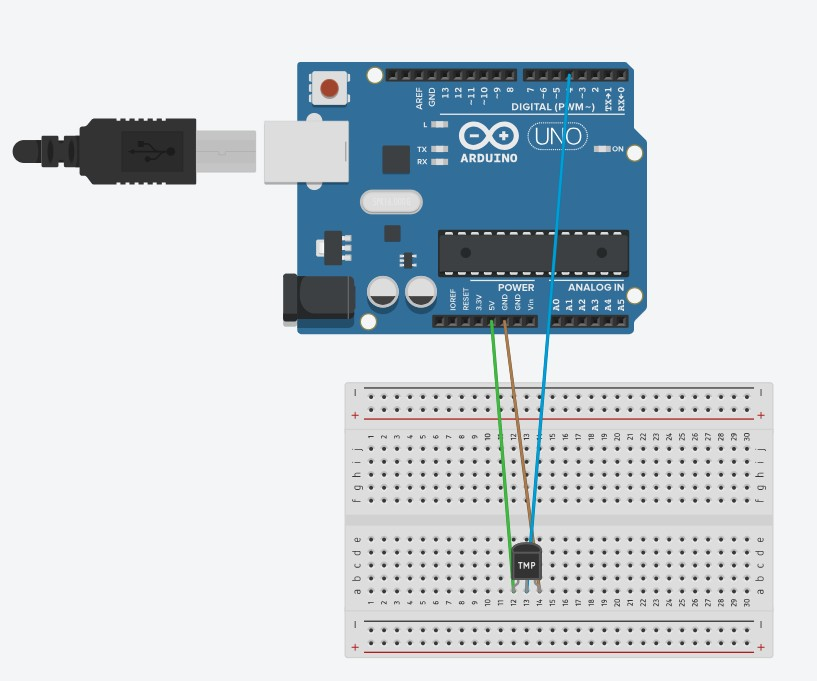
\includegraphics[width=0.50\linewidth]{img/diseno_dht.jpg}
    \caption{Circuito de conexión del sensor DHT-22 a la placa Arduino UNO.}
    \label{fig:diseno_dht}
\end{figure}
\pagebreak
%%%%%%%%%%%%%%%%%%%%%%%%%%%%%%%%%%%%%%%%%%%%%%%%%%%%%%%%%%%%%%%%%%%%%%%
\subsection{Actividad 6.2: Lectura del sensor}
\textit{Enunciado: Compile y suba el código 1 mostrado en los Anexos. Explique el
funcionamiento general del código. Adjunte capturas de pantalla en el informe. (2 puntos)}

El código del anexo se subió tal cual, con el único ajuste de las dos constantes que
describen el hardware utilizado (Código~\ref{lst:dht_pines}). El resto del código quedó
intacto.

\begin{lstlisting}[language=C++,
    caption={Ajuste de las constantes al hardware.},
    label={lst:dht_pines},
    float=ht!]
#define DHT_PIN       4        // Pin de datos del sensor
#define DHT_TYPE      DHT22    // Tipo de sensor disponible
\end{lstlisting}

\begin{figure}[ht!]
    \centering
    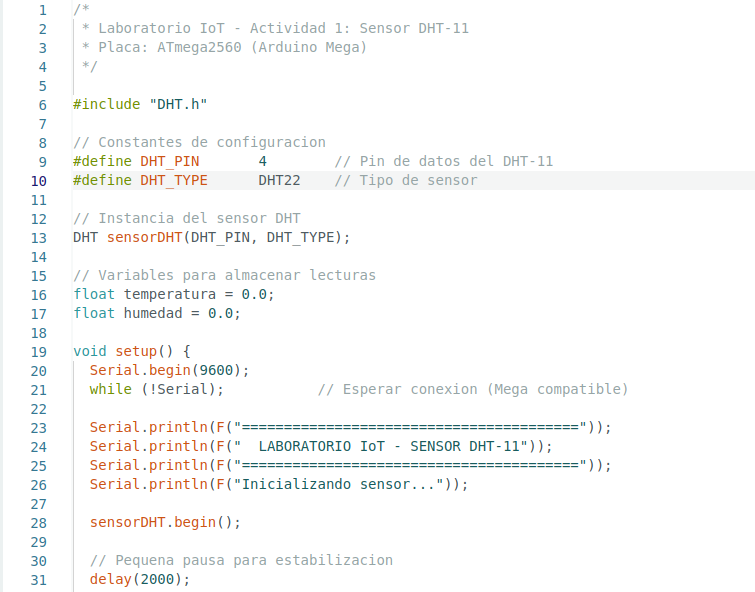
\includegraphics[width=0.85\linewidth]{img/sketch_dht.png}
    \caption{Código de lectura del sensor cargado en el IDE de Arduino.}
    \label{fig:sketch_dht}
\end{figure}

\pagebreak

El funcionamiento general es el siguiente. En \texttt{setup()} se abre el puerto serial a
9600~baudios, se inicializa el sensor con \texttt{sensorDHT.begin()} y se espera dos
segundos antes de la primera lectura, porque el DHT necesita ese tiempo para estabilizar
su circuito interno de medición.

El lazo \texttt{loop()} empieza con un \texttt{delay(2000)}. Esa pausa no es decorativa:
la frecuencia de muestreo del sensor es de 1~Hz, de modo que pedirle lecturas más seguido
devuelve el valor almacenado de la medición anterior en lugar de una lectura nueva.

Luego se llama a \texttt{readHumidity()} y \texttt{readTemperature()}, y el resultado se
valida con \texttt{isnan()} antes de usarlo. Esa validación es necesaria porque la
librería no lanza errores: cuando la trama de 40~bits llega corrupta o no llega, devuelve
un valor no numérico. Sin esa comprobación el programa seguiría imprimiendo basura como
si fueran mediciones válidas.

Con los datos ya validados se calcula el índice de calor mediante
\texttt{computeHeatIndex()}, que combina temperatura y humedad en la temperatura
aparente, y finalmente se imprime el bloque formateado junto con una clasificación por
umbrales, que marca la temperatura como alta por encima de $30^\circ$C y la humedad como
alta por encima de 70\,\%.

La Figura~\ref{fig:monitor_serial_dht} muestra cuatro ciclos consecutivos del monitor
serial. Las lecturas se mantuvieron alrededor de $26{,}0^\circ$C y 47\,\% de humedad
relativa, ambas dentro del rango normal según los umbrales del propio código.

\begin{figure}[ht!]
    \centering
    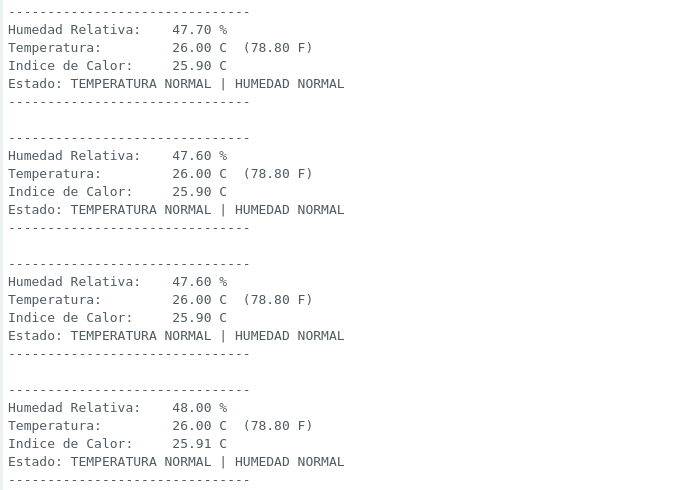
\includegraphics[width=0.8\linewidth]{img/monitor_serial_dht.png}
    \caption{Salida del monitor serial con las lecturas del sensor.}
    \label{fig:monitor_serial_dht}
\end{figure}

\clearpage
%%%%%%%%%%%%%%%%%%%%%%%%%%%%%%%%%%%%%%%%%%%%%%%%%%%%%%%%%%%%%%%%%%%%%%%
\subsection{Actividad 6.3: Lectura desde un script en Python}
\textit{Enunciado: Investigue de qué manera un script en Python puede obtener los datos que
el sensor DHT-11 escribe en el puerto serial. Programe en Python un ejemplo de uso que
muestre los datos del sensor, debe instalar en Python la librería \texttt{pyserial}.
(2 puntos)}

Esta actividad no se realizó en el laboratorio, sin embargo se investigó lo siguiente:
El microcontrolador no expone los datos de ninguna forma especial. Todo lo que hace es
escribir texto en el puerto serial con \texttt{Serial.println()}, y ese puerto, del lado
del PC, aparece como un archivo de dispositivo (\texttt{/dev/ttyUSB0} en el Linux Mint de
la mesa de trabajo). Lo que aporta \texttt{pyserial} es la capa que configura la velocidad,
la paridad y los tiempos de espera, y que entrega el flujo de bytes ya listo para
leer~\cite{pyserial}.

\clearpage
%%%%%%%%%%%%%%%%%%%%%%%%%%%%%%%%%%%%%%%%%%%%%%%%%%%%%%%%%%%%%%%%%%%%%%%
\section{Control de dispositivo de potencia}

%%%%%%%%%%%%%%%%%%%%%%%%%%%%%%%%%%%%%%%%%%%%%%%%%%%%%%%%%%%%%%%%%%%%%%%
\subsection{Actividad 6.5: Circuito de conexión del relé}
\textit{Enunciado: Muestre el circuito de conexión del Relé a la placa, utilice para ello
Fritzing. (1 punto)}

El montaje físico correspondiente quedó registrado en la
Figura~\ref{fig:diseno_rele} realizada con Tinkercad.

\begin{figure}[ht!]
    \centering
    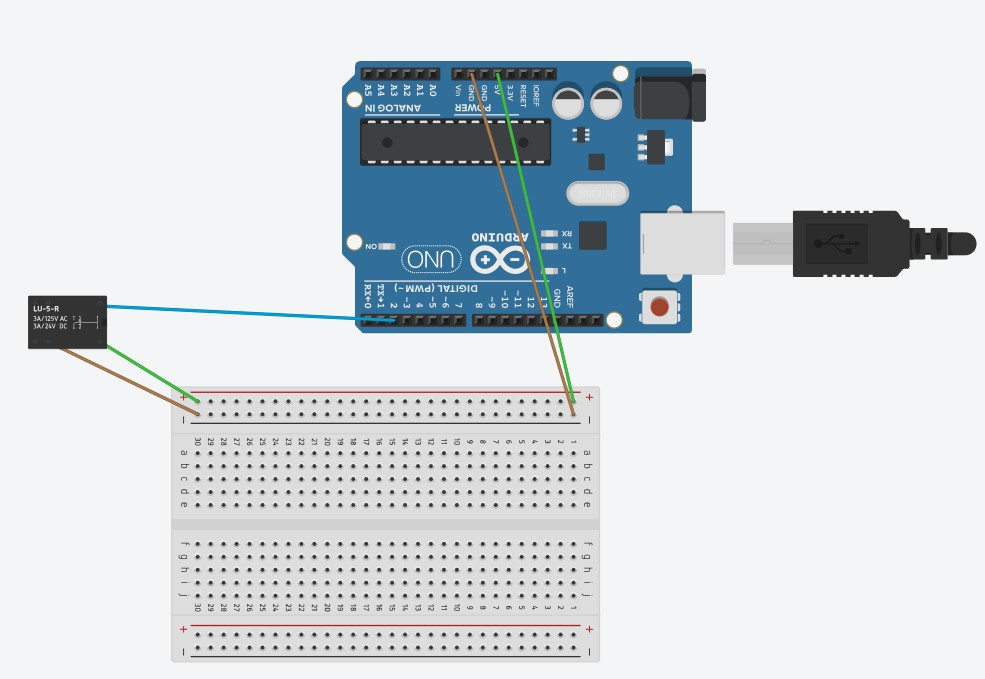
\includegraphics[width=0.50\linewidth]{img/diseno_rele.jpg}
    \caption{Circuito de conexión del relé a la placa Arduino UNO.}
    \label{fig:diseno_rele}
\end{figure}
\pagebreak

%%%%%%%%%%%%%%%%%%%%%%%%%%%%%%%%%%%%%%%%%%%%%%%%%%%%%%%%%%%%%%%%%%%%%%%
\subsection{Actividad 6.6: Control básico del relé}
\textit{Enunciado: Compile y suba el código 2 mostrado en los Anexos. Explique el
funcionamiento general del código. Adjunte capturas de pantalla en el informe. (2 puntos)}

El único ajuste al código del anexo fue mover el pin de control a digital~2, que es donde
quedó cableada la entrada \texttt{IN} del módulo.

El código hace dos cosas a la vez dentro de \texttt{loop()}. Por un lado mantiene una
secuencia automática de prueba que invierte el estado del relé cada cinco segundos, pero
lo hace comparando \texttt{millis()} contra una marca de tiempo anterior en lugar de usar
\texttt{delay()}. Esa distinción importa, porque \texttt{delay()} congelaría la placa
durante esos cinco segundos y no podría atender nada más. Por otro lado revisa en cada
vuelta si llegó un carácter por el puerto serial y, de ser así, lo despacha a
\texttt{procesarComando()}.

El detalle que más confunde de este montaje es que el módulo es activo en bajo. Escribir
\texttt{LOW} en el pin de control energiza la bobina y escribir \texttt{HIGH} la
desenergiza, que es lo contrario de lo que sugiere la intuición. El sketch lo resuelve con
el operador ternario \texttt{estadoRele ? LOW : HIGH}, y por eso el estado inicial seguro
en \texttt{setup()} es \texttt{HIGH}.

\begin{lstlisting}[language=C++,
    caption={Conmutación del relé y atención de comandos en \texttt{loop()}.},
    label={lst:rele_loop},
    float=ht!]
if (tiempoActual - tiempoAnterior >= INTERVALO_PRUEBA) {
    tiempoAnterior = tiempoActual;

    estadoRele = !estadoRele;
    cicloPrueba++;

    digitalWrite(PIN_RELE, estadoRele ? LOW : HIGH);  // Activo LOW
    digitalWrite(PIN_LED_IND, estadoRele ? HIGH : LOW);
}

if (Serial.available() > 0) {
    char comando = Serial.read();
    procesarComando(comando);
}
\end{lstlisting}

\clearpage
%%%%%%%%%%%%%%%%%%%%%%%%%%%%%%%%%%%%%%%%%%%%%%%%%%%%%%%%%%%%%%%%%%%%%%%
\subsection{Actividad 6.7: Relé con estado persistente}
\textit{Enunciado: Modifique el código para que el Relé mantenga el estado y solo se
modifique cuando se le indique a través del puerto serial. (2 puntos)}

La modificación consistió en eliminar por completo el bloque de la secuencia automática,
que era lo único que cambiaba el actuador por su cuenta. Sin ese bloque el lazo queda
reducido a atender comandos, y el relé conserva indefinidamente el último estado que se
le indicó.

Aprovechando el cambio se centralizó la escritura al hardware en una función
\texttt{aplicarEstado()}. En el sketch original cada rama del \texttt{switch} repetía las
dos llamadas a \texttt{digitalWrite()} junto con la asignación a \texttt{estadoRele}, y
ese patrón hace fácil que el estado lógico y el estado físico terminen desincronizados si
alguna rama se edita y otra no.

\begin{lstlisting}[language=C++,
    caption={Lazo principal y escritura centralizada, en \texttt{src/rele\_estado.ino}.},
    label={lst:rele_estado},
    float=ht!]
void loop() {
  // El lazo no toca el actuador, solo atiende comandos entrantes
  if (Serial.available() > 0) {
    char comando = Serial.read();
    procesarComando(comando);
  }
}

void aplicarEstado(bool encendido) {
  estadoRele = encendido;
  digitalWrite(PIN_RELE, encendido ? LOW : HIGH);   // Activo LOW
  digitalWrite(PIN_LED_IND, encendido ? HIGH : LOW);
}
\end{lstlisting}

Se agregaron además dos casos que ignoran \texttt{'\textbackslash r'} y
\texttt{'\textbackslash n'}. Sin ellos, el monitor serial configurado en modo
\textit{New Line} agrega el salto al final de cada envío y el sketch responde con el
mensaje de comando no reconocido después de cada orden válida.

%%%%%%%%%%%%%%%%%%%%%%%%%%%%%%%%%%%%%%%%%%%%%%%%%%%%%%%%%%%%%%%%%%%%%%%
\subsection{Actividad 6.8: Consulta y control del relé desde Python}
\textit{Enunciado: Investigue de qué manera un script en Python podría leer el estado
actual del Relé y adicionalmente enviar comandos a la placa para modificar el estado del
actuador. Programe en Python un ejemplo de uso, debe instalar en Python la librería
\texttt{pyserial}. (2 puntos)}

Esta actividad no se realizó en el laboratorio, sin embargo se investigó lo siguiente:
La clave está en que el puerto serial es bidireccional, de modo que el mismo enlace que se
usa para leer sirve para escribir. El código ya define un protocolo
mínimo de un carácter por comando, así que del lado de Python basta con escribir ese
carácter y leer las líneas que la placa devuelva.

\clearpage
%%%%%%%%%%%%%%%%%%%%%%%%%%%%%%%%%%%%%%%%%%%%%%%%%%%%%%%%%%%%%%%%%%%%%%%
\section{Automatización mediante sensor y actuador}

%%%%%%%%%%%%%%%%%%%%%%%%%%%%%%%%%%%%%%%%%%%%%%%%%%%%%%%%%%%%%%%%%%%%%%%
\subsection{Actividad 6.10: Circuito con sensor y actuador}
\textit{Enunciado: Muestre el circuito de conexión que incluya al sensor y al actuador,
utilice para ello Fritzing. (1 punto)}

El montaje físico correspondiente quedó registrado en la
Figura~\ref{fig:diseno_dht_rele} realizada con Tinkercad.

\begin{figure}[ht!]
    \centering
    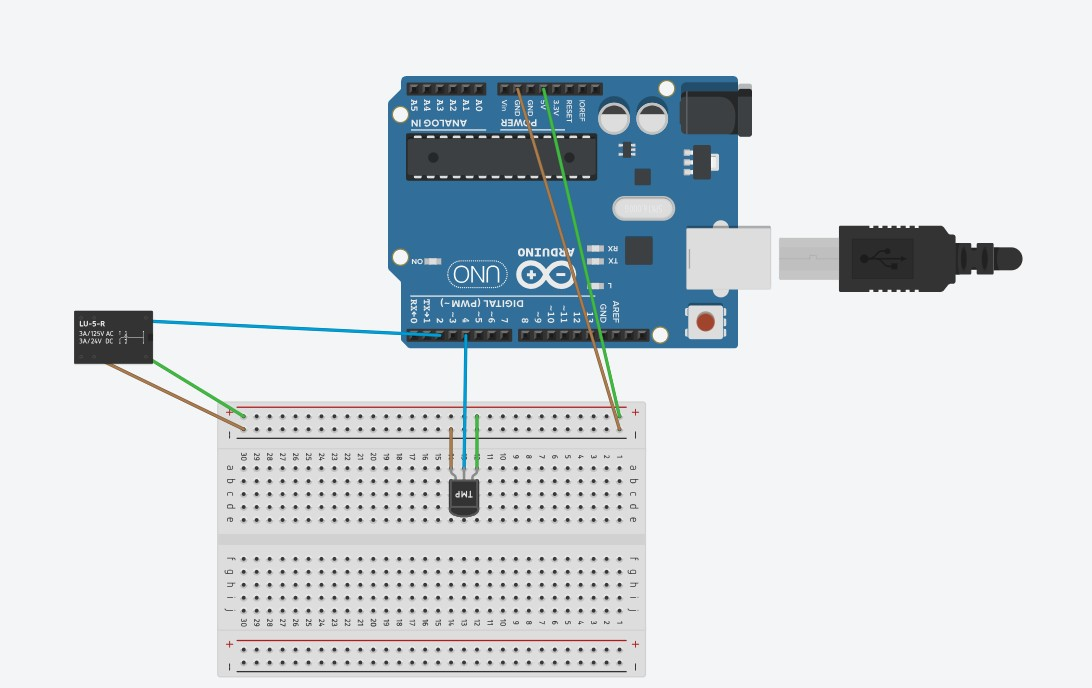
\includegraphics[width=0.50\linewidth]{img/diseno_dht_rele.jpg}
    \caption{Circuito de conexión del DHT y relé a la placa Arduino UNO.}
    \label{fig:diseno_dht_rele}
\end{figure}
\pagebreak

El montaje final integró los dos elementos sobre la misma placa. El sensor quedó en la
protoboard con su línea de datos hacia el pin~4, y el módulo de relé recibió la señal de
control en el pin~2, con la alimentación de ambos tomada de los rieles de 5~V y GND
(Figuras~\ref{fig:montaje_dht_rele} y~\ref{fig:montaje_angulo}).

\begin{figure}[ht!]
    \centering
    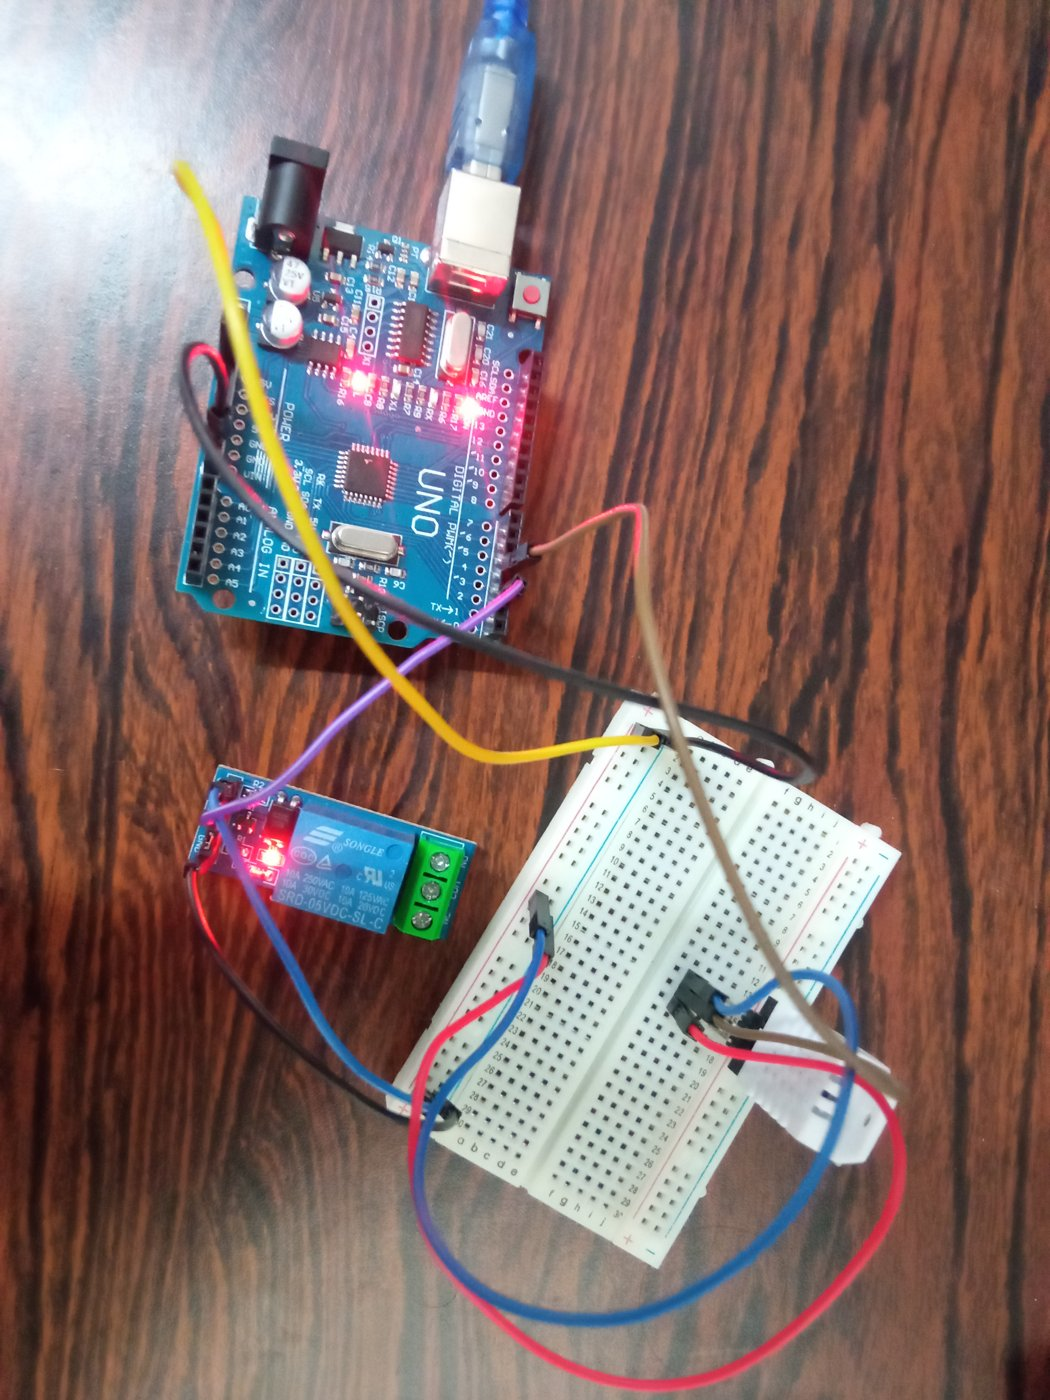
\includegraphics[width=0.52\linewidth]{img/montaje_dht_rele.jpg}
    \caption{Montaje del sensor y el relé sobre la Arduino UNO.}
    \label{fig:montaje_dht_rele}
\end{figure}

\pagebreak

\begin{figure}[ht!]
    \centering
    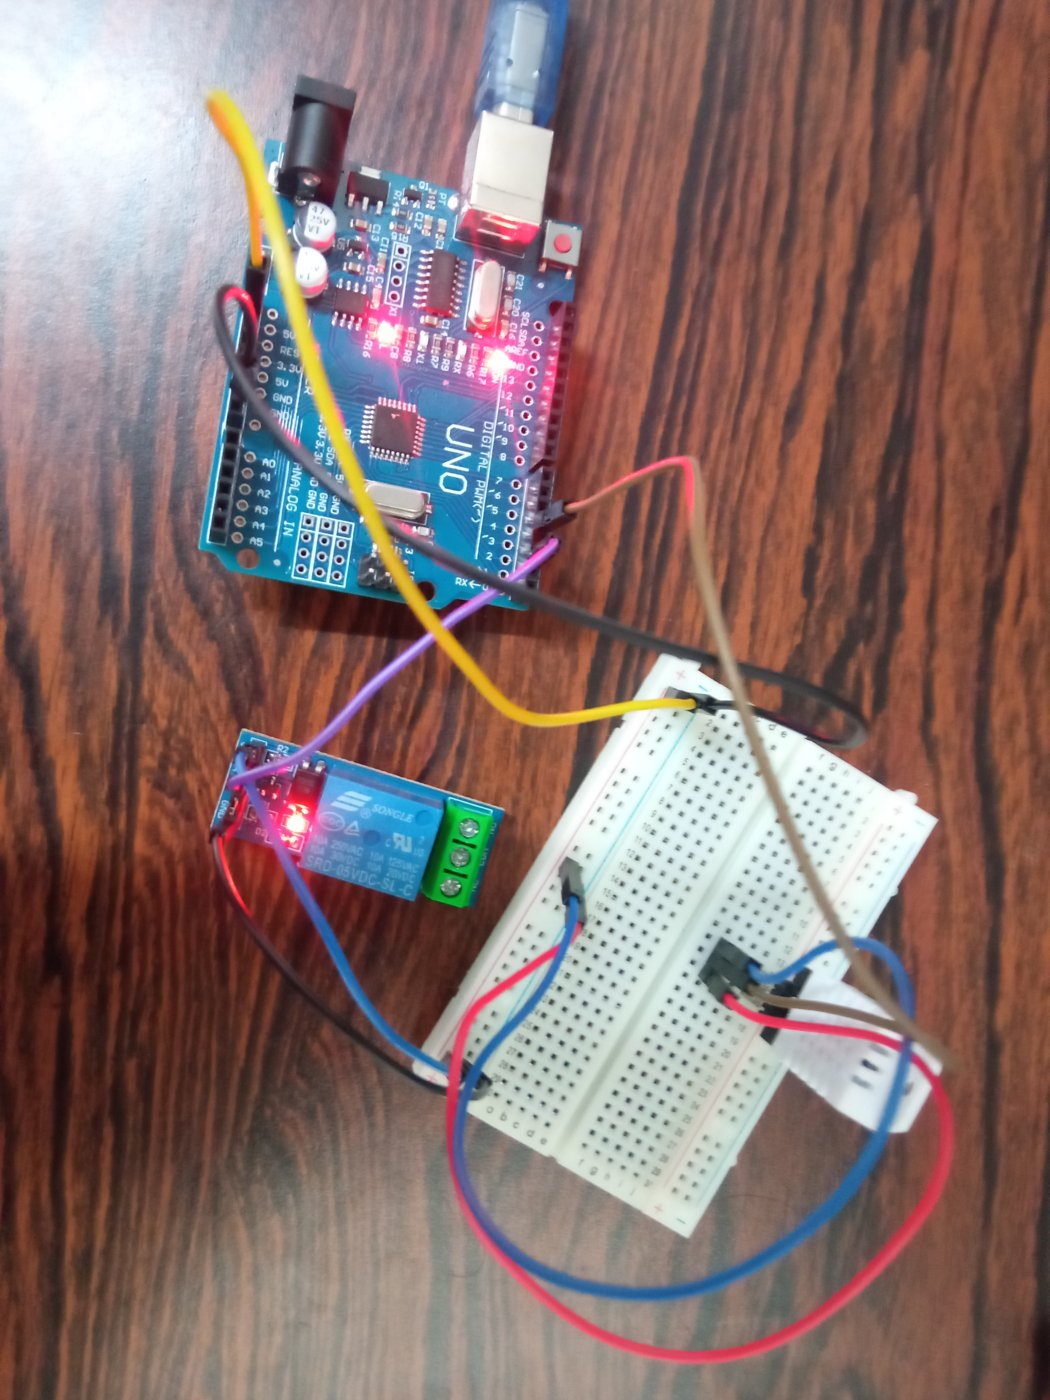
\includegraphics[width=0.52\linewidth]{img/montaje_dht_rele_angulo.jpg}
    \caption{Segunda vista del montaje, con el cableado de control y alimentación.}
    \label{fig:montaje_angulo}
\end{figure}

%%%%%%%%%%%%%%%%%%%%%%%%%%%%%%%%%%%%%%%%%%%%%%%%%%%%%%%%%%%%%%%%%%%%%%%
\subsection{Actividad 6.11: Automatización por umbrales}
\textit{Enunciado: Programe, en el ATmega2560, el código para que el Relé mantenga el
estado y solo se modifique cuando se le indique a través del puerto serial. (2 puntos)}

El sketch resultante combina las dos mitades anteriores. Lee temperatura y humedad cada
dos segundos, las compara contra dos umbrales configurables y acciona el relé cuando
cualquiera de los dos se supera. Basta con que una de las dos variables se salga de rango para que el actuador se
active (Código~\ref{lst:integrado}).

\begin{lstlisting}[language=C++,
    caption={Lógica de control por umbrales, en \texttt{src/dht11\_rele.ino}.},
    label={lst:integrado},
    float=ht!]
float limiteTemperatura = 30.0;
float limiteHumedad = 60.0;

if (temperatura >= limiteTemperatura || humedad >= limiteHumedad) {
    digitalWrite(PIN_RELE, LOW);    // Activa el rele
    Serial.println(F("-> ALERTA: Limite superado (Temp o Hum). Rele ENCENDIDO."));
} else {
    digitalWrite(PIN_RELE, HIGH);   // Apaga el rele
    Serial.println(F("-> Condiciones normales. Rele APAGADO."));
}
\end{lstlisting}

\begin{figure}[ht!]
    \centering
    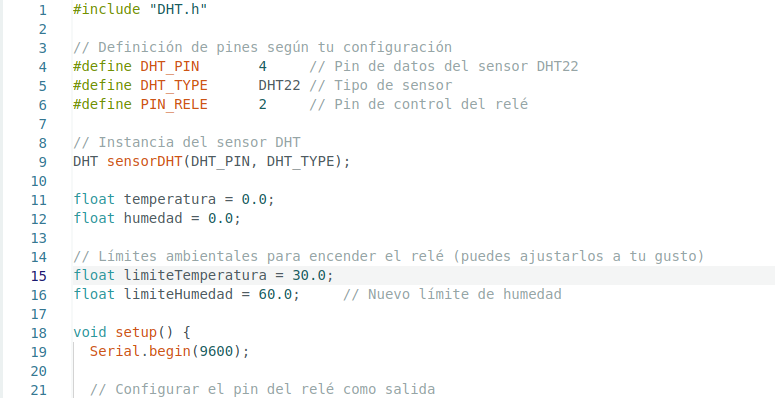
\includegraphics[width=0.85\linewidth]{img/sketch_integrado.png}
    \caption{Sketch integrado cargado en el IDE, con los umbrales configurados.}
    \label{fig:sketch_integrado}
\end{figure}

\pagebreak

El umbral de humedad se ajustó durante la prueba de 70\,\% a 60\,\% para acercarlo a
las condiciones del salón, donde las lecturas rondaban el 50\,\%. Aun así no se alcanzó
a cruzar el umbral, de modo que la Figura~\ref{fig:monitor_serial_integrado} documenta la
rama de condiciones normales con el relé apagado, que es el comportamiento correcto para
esos valores.

\begin{figure}[ht!]
    \centering
    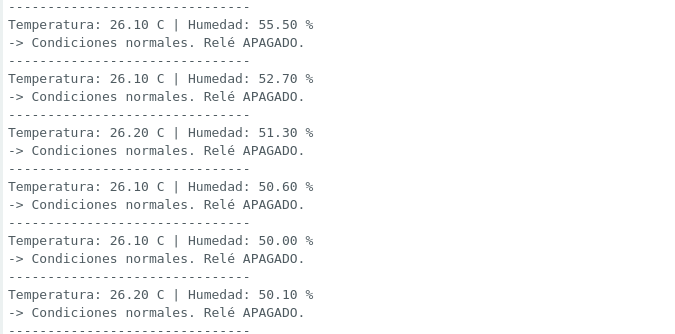
\includegraphics[width=0.8\linewidth]{img/monitor_serial_integrado.png}
    \caption{Telemetría del sistema integrado con el relé en reposo.}
    \label{fig:monitor_serial_integrado}
\end{figure}

\clearpage
%%%%%%%%%%%%%%%%%%%%%%%%%%%%%%%%%%%%%%%%%%%%%%%%%%%%%%%%%%%%%%%%%%%%%%%
\section{Conclusiones}

El laboratorio dejó claro que trabajar con un sensor digital no se reduce a leer un
valor. El DHT entrega una trama de 40~bits que puede llegar corrupta, y la librería
señala esa falla devolviendo un valor no numérico en lugar de lanzar un error. La
validación con \texttt{isnan()} no es una precaución opcional, es lo único que separa una
medición real de un dato sin sentido.

Del lado del actuador, el punto que más costó asimilar fue la lógica invertida del módulo
de relé. Un módulo activo en bajo se energiza escribiendo \texttt{LOW}, de modo que el
estado seguro al arrancar es \texttt{HIGH}. Fijar ese estado en \texttt{setup()} evita que
la carga quede conectada durante el arranque de la placa.

Separar el estado lógico del estado físico resultó ser la decisión más útil del
laboratorio. Concentrar las llamadas a \texttt{digitalWrite()} en una sola función hace
imposible que una rama del código cambie el actuador sin actualizar la variable que lo
describe, que es justamente el error que después Python no podría detectar cuando consulta
el estado por el puerto serial.

Finalmente, la automatización por umbrales mostró el esquema completo de un sistema IoT
sencillo: el sensor entrega el dato, la lógica en el microcontrolador decide y el actuador
ejecuta, todo sin intervención del PC. El PC queda solo como observador a través del
puerto serial, que es exactamente la separación entre la lógica de interfaz y la ejecución
en hardware que plantea la introducción de la guía.

\clearpage
%%%%%%%%%%%%%%%%%%%%%%%%%%%%%%%%%%%%%%%%%%%%%%%%%%%%%%%%%%%%%%%%%%%%%%%
\begingroup
\small
\begin{thebibliography}{9}

\bibitem{dhtlib}
Adafruit Industries, ``DHT-sensor-library,'' \emph{GitHub Repository}, 2012--2024.
[En línea]. Disponible: \url{https://github.com/adafruit/DHT-sensor-library}.
[Consulta: sep.~2026]

\bibitem{aosong}
Aosong Electronics, ``DHT22 (AM2302) Digital-output relative humidity and temperature
sensor,'' hoja de datos técnica, 2024. [En línea]. Disponible:
\url{https://www.sparkfun.com/datasheets/Sensors/Temperature/DHT22.pdf}.
[Consulta: sep.~2026]

\bibitem{pyserial}
C.~Liechti, ``pySerial Documentation,'' 2001--2024. [En línea]. Disponible:
\url{https://pyserial.readthedocs.io/en/latest/}. [Consulta: sep.~2026]

\bibitem{arduinoref}
Arduino, ``Arduino Language Reference,'' \emph{Arduino Documentation}, Arduino LLC, 2024.
[En línea]. Disponible: \url{https://docs.arduino.cc/language-reference/}.
[Consulta: sep.~2026]

\bibitem{guialab}
A.~Russoniello, ``Laboratorio: Sensores y Actuadores,'' guía de práctica de laboratorio,
Laboratorio General (Internet de las Cosas), Escuela de Computación,
Facultad de Ciencias, Universidad Central de Venezuela, Caracas, 2026.

\end{thebibliography}
\endgroup

\end{document}
